Carry Look-Ahead Adder (CLA) là một loại bộ cộng số học trong kỹ thuật số, được thiết kế để thực hiện phép cộng hai số nhị phân nhanh hơn so với bộ cộng thông thường (như Ripple Carry Adder - RCA). CLA đạt được tốc độ cao bằng cách tính toán các tín hiệu carry đồng thời (song song) thay vì tuần tự, nhờ vào các tín hiệu Generate (G) và Propagate (P). 

\begin{figure}[H]
	\centering
	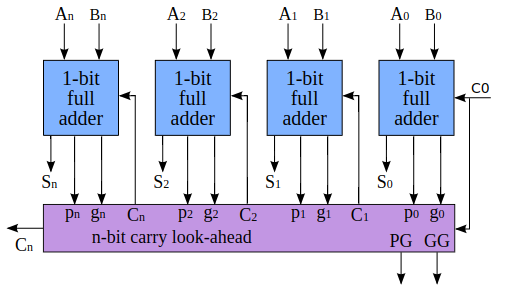
\includegraphics[width=0.5\linewidth]{./image/carry_look_ahead_structure.png}
	\caption{Cấu trúc của bộ Carry Look-Ahead}
	\label{f_carry look ahead structure}
\end{figure}

Trong đó,

\begin{itemize}[label = -]
	\item Generate $(G_{i})$: $G_{i} = A_{i} \cdot B_{i} $i.
	\item Propagate $(P_{i})$: $P_{i} = A_{i} + B_{i}$.
	\item Tổng $(S_{i})$: $S_{i} = G_{i} \cdot P_{i}$.
	\item Carry $(C_{i+1})$: $C_{i + 1} = G_{i} + P_{i}\cdot C_{i}$.
\end{itemize}

\begin{itemize}[label = -]
	\item Ưu điểm: 
	\begin{itemize}[label = +]
		\item Tốc độ xử lý cao do tín hiệu carry được xử lý song song.
		\item Giảm độ trễ với độ trễ tăng theo $O(\log_{2}(n))$, thay vì $O(n)$ như RCA.
	\end{itemize}
	\item Nhược điểm:
	\begin{itemize}[label = +]
		\item Phức tạp về thiết kế do yêu cầu xử dụng nhiều cổng logic để tính toán carry đồng thời, làm tăng độ phức tạp của hệ thống.
		\item Tốn tài nguyên phần cứng do số lượng cổng logic tăng nhanh khi số bit tăng, làm tăng chi phí phần cứng.
		\item Khó mở rộng do khi số bit lớn thì yêu cầu cần thiết kế phức tạp hơn, và việc tính toán carry đòi hỏi nhiều tài nguyên.
	\end{itemize}
\end{itemize}

\begin{lstlisting}[style = SystemVerilog, caption={CLA}]
	module cla (
	input  logic [31:0] i_data_a,   // Operand A (32-bit input)
	input  logic [31:0] i_data_b,   // Operand B (32-bit input)
	output logic [31:0] o_data,     // Sum output (32-bit)
	output logic        o_carry     // Carry-out (1-bit output)
	);
	logic [31:0] G, P;              // Bitwise Generate (G) and Propagate (P) signals
	logic [32:0] C;                 // Carry signals for each bit (including carry-out)
	
	// Generate and Propagate logic
	// G[i] = i_data_a[i] & i_data_b[i]: A carry is generated when both bits are 1.
	// P[i] = i_data_a[i] | i_data_b[i]: A carry is propagated if at least one of the bits is 1.
	assign G = i_data_a & i_data_b; // Generate signals
	assign P = i_data_a | i_data_b; // Propagate signals
	
	// Carry logic
	// C[0] is initialized to 0 because there is no carry-in for the least significant bit.
	// C[i+1] = G[i] | (P[i] & C[i]): Carry for the next bit depends on the current bit's generate or propagate conditions.
	assign C[0] = 0; // Initial carry-in is 0
	generate
	genvar i;
	for (i = 0; i < 32; i++) begin : carry_logic_block
	// Compute carry-out for each bit position
	assign C[i+1] = G[i] | (P[i] & C[i]);
	end
	endgenerate
	
	// Sum logic
	// o_data[i] = i_data_a[i] ^ i_data_b[i] ^ C[i]: The sum is computed using the XOR of the two operands and the carry-in for each bit.
	assign o_data = i_data_a ^ i_data_b ^ C[31:0]; // Sum computation
	assign o_carry = C[32]; // The final carry-out from the most significant bit
	endmodule
\end{lstlisting}

\begin{lstlisting}[style=C, caption={Kết quả test}]
	$ ./obj_dir/Vcla 
	=== Test bench for Ripple Carry Adder (RCA) ===
	[PASS] Test case 1: A = 234, B = 25, Expected = 259, Actual = 259
	[PASS] Test case 2: A = 30, B = 255, Expected = 285, Actual = 285
	[PASS] Test case 3: A = 120, B = 28, Expected = 148, Actual = 148
	[PASS] Test case 4: A = 194, B = 123, Expected = 317, Actual = 317
	...
	[PASS] Test case 99: A = 85, B = 175, Expected = 260, Actual = 260
	[PASS] Test case 100: A = 101, B = 30, Expected = 131, Actual = 131
	
	=== Test Summary ===
	Total Test Cases: 100
	PASS: 100
	FAIL: 0
\end{lstlisting}